I have simulated 1000000 repetitions of the experiment of drawing 20 i.i.d Bernoulli random variables $X_1,...,X_{20}$ with bias $\frac{1}{2}$, and plotted the empirical frequency of observing $\overline{X} = \frac{1}{20}\sum_{i=1}^{20}X_i \geq \alpha$ for $\alpha \in \{0.5,0.55,...,0.95,1.0 \}$. It is clear that since we only draw 20 random variables, and all of them have a value of 0 or 1, then the $\overline{X}$ will be a multiple of $0.05$ between 0 and 1. Therefore, it would not provide additional information to choose a finer granularity of $\alpha$ than the chosen one. Here is my plot:

\begin{center}
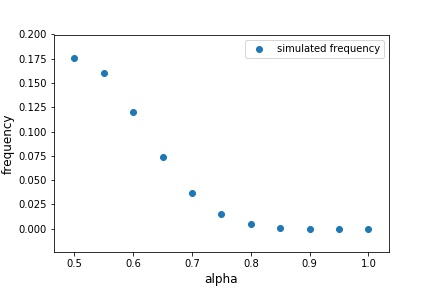
\includegraphics[scale = 0.7]{illustration_of_hoeffding/fig1.jpg}
\end{center}

As expected from the bias of each $X_i$ being $\frac{1}{2}$, the simulated frequency becomes lower and lower the further from $0.5$ the value of $\alpha$ becomes. Due to the central limit theorem and the fact that we are simulating a big number of experiments, we should in fact be observing something that approximates the right half of a normal distribution with mean $0.5$. This corresponds well with the actual plot.

By substituting $\epsilon = \alpha - \mu$ and $\mathbb{E}(X_i) = \mu$ in the formulation of Hoeffding's Inequality in \textbf{corrolary 2.4}, we get:
\begin{align}
\mathbb{P}\left( \sum_{i=1}^n X_i - n\mu \geq \alpha - \mu \right  ) \leq e^{2n(\alpha - \mu)^2}
\end{align}
which is equivalent to
\begin{align}
\mathbb{P}\left( \overline{X} \geq \alpha \right  ) \leq e^{2n(\alpha - \mu)^2}
\end{align}
By setting $\mu = 0.5$, we can use this formula to calculate the Hoeffding bound on the probability of observing $\overline{X} \geq \alpha$ as a function of $\alpha$. Here is my plot of this bound and the simulated frequency of the event actually happening:
\begin{center}
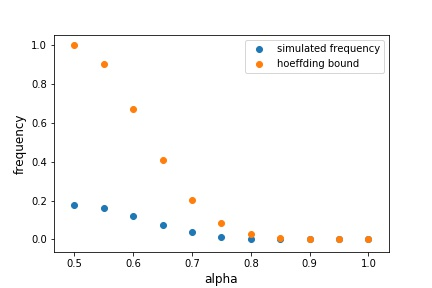
\includegraphics[scale = 0.7]{illustration_of_hoeffding/fig2.jpg}
\end{center}
As expected, we see that the bound is always larger than the simulated frequency. We also see that the larger $\alpha$ becomes, the tighter the Hoeffding also becomes compared to the simulated frequency.

By substituting $\epsilon = \alpha$ and $\mathbb{E}(X_i) = 0.5$ in the formulation of Markov Inequality in \textbf{corrolary 2.1}, we can calculate the Markov bound on the probability of observing $\overline{X} \geq \alpha$ as a function of $\alpha$. Here is my plot:

\begin{center}
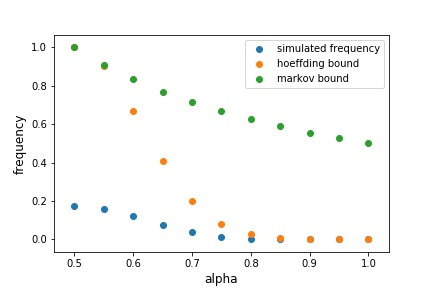
\includegraphics[scale = 0.7]{illustration_of_hoeffding/fig3.jpg}
\end{center}

From this plot, we can see that Hoeffdings Inequality gives tighter bounds than Markovs Inequality.

We can calculate the probability that $\overline{X} = 1$ as 
\begin{align}
P(\overline{X} = 1) = \left( \frac{1}{2} \right)^{20} \approx 9.54 \cdot 10^{-7}
\end{align}
The Hoeffding bound on this probability is approximately $4.54 \cdot 10^{-5}$.

Using the binomial distribution, we can find the probability getting 1 or 0 successes on 20 tries with 0.5 success probability on each try. This is equivalent to the probability of $\overline{X} \geq 0.95$. The probability is approximately $2.01 \cdot 10^{-5}$. The Hoeffding bound on this probability is approximately $3.03 \cdot 10^{-4}$.